%%%%%%%%%% EJERCICIO 2 %%%%%%%%%%

\begin{ejer}
    \textbf{Ejercicio 2. Un ejemplo clásico de red social de tamaño pequeño es el de las familias 
    más influyentes en la política, la economía y la vida social de la Florencia del siglo XV. 
    Los historiadores John Padgett y Christopher Ansell estudiaron esta red social en 1993, 
    basándose en datos tomados de archivos históricos (ver el artículo [2], que se ha adjuntado en 
    Recursos del aula virtual). El grafo que representa dicha red social, que no es dirigido, 
    y se forma dibujando una arista entre dos familias cada vez que un matrimonio las vincula, es el siguiente:}
\end{ejer}
\addcontentsline{toc}{subsection}{Ejercicio 2}
 %%% IMAGEN DE FAMILIAS INFLUYENTES %%%
 \begin{figure}[H]
	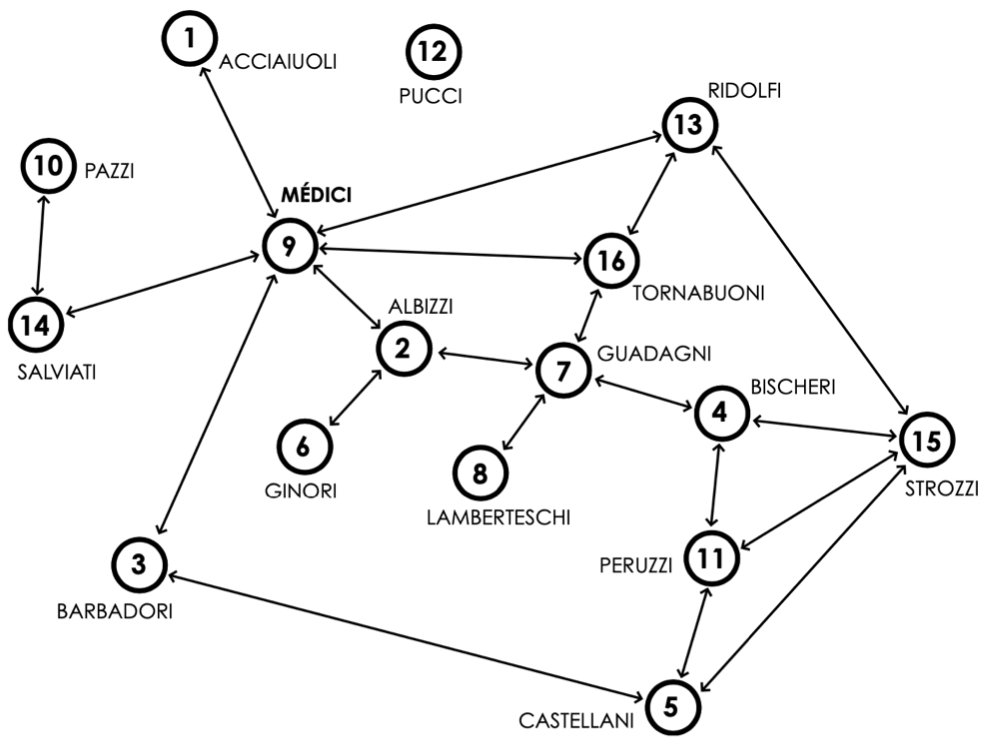
\includegraphics[width=\textwidth/2]{familiasInfluyentes}
	\centering
	\caption{Familias influyentes de Florencia.}
    \label{fig:familiasInfluyentes}
\end{figure}
\begin{ejer}
    \textbf{A simple vista se observa que la familia Médici, con el vértice $9$, ocupa una posición central, pues ostenta el grado máximo. 
    Los autores del estudio conjeturaron que los Médici alcanzaron una posición de dominio en la sociedad florentina precisamente forzando 
    su alianza con el resto de familias a través de múltiples matrimonios.}
\end{ejer}
%%%%%%%%%%%%%%%%%%%%%%%%%%%%%%%%%%%%%%%%%%%%%%%%%%%%%%%    APARTADO_1   %%%%%%%%%%%%%%%%%%%%%%%%%%%%%%%%%%%%%%%%%%%%%%%%%%%%%%%%%%%%%%%
\begin{ejer}
    \begin{itemize}
        \item \textbf{Aplica el algoritmo PageRank a esta red social para confirmar que, en efecto, la familia Médici era la más relevante en esta pequeña red social.}
    \end{itemize}
\end{ejer}
\addcontentsline{toc}{subsubsection}{Apartado 1}
\begin{sagecommandline}
    sage: N = matrix(RDF,[[0, 0, 0, 0, 0, 0, 0, 0, 1, 0, 0, 0, 0, 0, 0, 0],[0, 0, 0, 0, 0, 1/3, 1/3, 0, 1/3, 0, 0, 0, 0, 0, 0, 0],[0, 0, 0, 0, 1/2, 0, 0, 0, 1/2, 0, 0, 0, 0, 0, 0, 0],[0, 0, 0, 0, 0, 0, 1/3, 0, 0, 0, 1/3, 0, 0, 0, 1/3, 0],[0, 0, 1/3, 0, 0, 0, 0, 0, 0, 0, 1/3, 0, 0, 0, 1/3, 0],[0, 1, 0, 0, 0, 0, 0, 0, 0, 0, 0, 0, 0, 0, 0, 0],[0, 1/4, 0, 1/4, 0 , 0, 0, 1/4, 0, 0, 0, 0, 0, 0, 0,1/4],[0, 0, 0, 0, 0, 0, 1, 0, 0, 0, 0, 0, 0, 0, 0, 0],[1/6, 1/6, 1/6, 0, 0 , 0, 0, 0, 0, 1/6, 0, 0, 1/6, 1/6, 0, 0],[0, 0, 0, 0, 0, 0, 0, 0, 0, 0, 0, 0, 0, 1, 0, 0],[0, 0, 0, 1/2, 1/2 , 0, 0, 0, 0, 0, 0, 0, 0, 0, 0, 0],[0, 0, 0, 0, 0, 0, 0, 0, 0, 0, 0, 0, 0, 0, 0, 0],[0, 0, 0, 0, 0, 0, 0, 0, 1/3, 0, 0, 0, 0, 0, 1/3, 1/3],[0, 0, 0, 0, 0, 0, 0, 0, 1/2, 1/2, 0, 0, 0, 0, 0, 0],[0, 0, 0, 1/4, 1/4, 0, 0, 0, 0, 0, 1/4, 0, 1/4, 0, 0, 0],[0, 0, 0, 0, 0, 0, 1/3, 0, 1/3, 0, 0, 0, 1/3, 0, 0, 0]])
\end{sagecommandline}
\resizebox{\textwidth}{!}{$
    N(x)= \sage{N}
$}
\par $N(x)$ representa la matriz de transición de la red descrita anteriormente.

\par El primer paso es crear una matriz estocástica $Q(x)$, que sirve para asegurarnos de que el camino
aleatorio llega a todas las familias de la red social. Para ello, observo la matriz inicial y añado en la fila
que no tiene ningún enlace de salida (por tanto un nodo colgante) el valor $1/n^o nodos$ a todas sus columnas para indicar que 
a todos los nodos, incluido el mismo, se puede llegar con la misma aleatoridad y de manera uniforme. 

\newpage

\begin{sagecommandline}
    sage: Q = matrix(RDF,[[0, 0, 0, 0, 0, 0, 0, 0, 1, 0, 0, 0, 0, 0, 0, 0],[0, 0, 0, 0, 0, 1/3, 1/3, 0, 1/3, 0, 0, 0, 0, 0, 0, 0],[0, 0, 0, 0, 1/2, 0, 0, 0, 1/2, 0, 0, 0, 0, 0, 0, 0],[0, 0, 0, 0, 0, 0, 1/3, 0, 0, 0, 1/3, 0, 0, 0, 1/3, 0],[0, 0, 1/3, 0, 0, 0, 0, 0, 0, 0, 1/3, 0, 0, 0, 1/3, 0],[0, 1, 0, 0, 0, 0, 0, 0, 0, 0, 0, 0, 0, 0, 0, 0],[0, 1/4, 0, 1/4, 0 , 0, 0, 1/4, 0, 0, 0, 0, 0, 0, 0,1/4],[0, 0, 0, 0, 0, 0, 1, 0, 0, 0, 0, 0, 0, 0, 0, 0],[1/6, 1/6, 1/6, 0, 0 , 0, 0, 0, 0, 1/6, 0, 0, 1/6, 1/6, 0, 0],[0, 0, 0, 0, 0, 0, 0, 0, 0, 0, 0, 0, 0, 1, 0, 0],[0, 0, 0, 1/2, 1/2 , 0, 0, 0, 0, 0, 0, 0, 0, 0, 0, 0],[1/16, 1/16, 1/16, 1/16, 1/16, 1/16, 1/16, 1/16, 1/16, 1/16, 1/16, 1/16, 1/16, 1/16, 1/16, 1/16],[0, 0, 0, 0, 0, 0, 0, 0, 1/3, 0, 0, 0, 0, 0, 1/3, 1/3],[0, 0, 0, 0, 0, 0, 0, 0, 1/2, 1/2, 0, 0, 0, 0, 0, 0],[0, 0, 0, 1/4, 1/4, 0, 0, 0, 0, 0, 1/4, 0, 1/4, 0, 0, 0],[0, 0, 0, 0, 0, 0, 1/3, 0, 1/3, 0, 0, 0, 1/3, 0, 0, 0]])
\end{sagecommandline}
\resizebox{\textwidth}{!}{$
    Q(x)= \sage{Q}
$}

\par El segundo paso, es obtener la matriz de transición de PageRank $P=pQ + (1-p)A$ para resolver el 
problema de que se atasque en pequeños subgrafos de la red.
\par Donde:
\begin{itemize}
    \item $Q$ es la matriz obtenida en el paso anterior.
    \item $A$ es la matriz ($n^onodos \times n^onodos$), donde todos los nodos están conectados entre sí y cuyas 
    entradas son $1/n^o nodos$.
    \begin{sagecommandline}
        sage: A = matrix(RDF,[[1/16, 1/16, 1/16, 1/16, 1/16, 1/16, 1/16, 1/16, 1/16, 1/16, 1/16, 1/16, 1/16, 1/16, 1/16, 1/16],[1/16, 1/16, 1/16, 1/16, 1/16, 1/16, 1/16, 1/16, 1/16, 1/16, 1/16, 1/16, 1/16, 1/16, 1/16, 1/16],[1/16, 1/16, 1/16, 1/16, 1/16, 1/16, 1/16, 1/16, 1/16, 1/16, 1/16, 1/16, 1/16, 1/16, 1/16, 1/16],[1/16, 1/16, 1/16, 1/16, 1/16, 1/16, 1/16, 1/16, 1/16, 1/16, 1/16, 1/16, 1/16, 1/16, 1/16, 1/16],[1/16, 1/16, 1/16, 1/16, 1/16, 1/16, 1/16, 1/16, 1/16, 1/16, 1/16, 1/16, 1/16, 1/16, 1/16, 1/16],[1/16, 1/16, 1/16, 1/16, 1/16, 1/16, 1/16, 1/16, 1/16, 1/16, 1/16, 1/16, 1/16, 1/16, 1/16, 1/16],[1/16, 1/16, 1/16, 1/16, 1/16, 1/16, 1/16, 1/16, 1/16, 1/16, 1/16, 1/16, 1/16, 1/16, 1/16, 1/16],[1/16, 1/16, 1/16, 1/16, 1/16, 1/16, 1/16, 1/16, 1/16, 1/16, 1/16, 1/16, 1/16, 1/16, 1/16, 1/16],[1/16, 1/16, 1/16, 1/16, 1/16, 1/16, 1/16, 1/16, 1/16, 1/16, 1/16, 1/16, 1/16, 1/16, 1/16, 1/16],[1/16, 1/16, 1/16, 1/16, 1/16, 1/16, 1/16, 1/16, 1/16, 1/16, 1/16, 1/16, 1/16, 1/16, 1/16, 1/16],[1/16, 1/16, 1/16, 1/16, 1/16, 1/16, 1/16, 1/16, 1/16, 1/16, 1/16, 1/16, 1/16, 1/16, 1/16, 1/16],[1/16, 1/16, 1/16, 1/16, 1/16, 1/16, 1/16, 1/16, 1/16, 1/16, 1/16, 1/16, 1/16, 1/16, 1/16, 1/16],[1/16, 1/16, 1/16, 1/16, 1/16, 1/16, 1/16, 1/16, 1/16, 1/16, 1/16, 1/16, 1/16, 1/16, 1/16, 1/16],[1/16, 1/16, 1/16, 1/16, 1/16, 1/16, 1/16, 1/16, 1/16, 1/16, 1/16, 1/16, 1/16, 1/16, 1/16, 1/16],[1/16, 1/16, 1/16, 1/16, 1/16, 1/16, 1/16, 1/16, 1/16, 1/16, 1/16, 1/16, 1/16, 1/16, 1/16, 1/16],[1/16, 1/16, 1/16, 1/16, 1/16, 1/16, 1/16, 1/16, 1/16, 1/16, 1/16, 1/16, 1/16, 1/16, 1/16, 1/16]])
    \end{sagecommandline} 
    \resizebox{\textwidth}{!}{$
        A(x)= \sage{A}
    $}
    \begin{sagecommandline}
        sage: GA = Graph(A, multiedges=True)
        sage: Aplot = GA.plot()
    \end{sagecommandline}
    
    %%% GRAFO DE RED SIMPLIFICADA %%%
    \begin{figure}[H]
        \sageplot[scale=.6]{Aplot, axes=False}
        \centering
        \label{redA_2}
        \caption{Red A donde todos los nodos están conectados entre sí.}
    \end{figure}
    \item $p$ es el factor de amortiguamiento propuesto por Brin y Page (1998) que tiene que ser un valor 
    comprendido entre [0..1], en este caso particular Google estableció $p=0.85$.
    \begin{sagecommandline}
        sage: factor=0.85
    \end{sagecommandline}
    \item  $(1-p)$ es la probabilidad de que un internauta decida no seguir ningún enlace en la página y 
    navegar a una nueva y aleatoria dentro de la red. Por otro lado, con probabilidad $p$, sigue los enlaces de 
    la página como de costumbre.
    \begin{sagecommandline}
        sage: prob_nueva_pagina=1-factor
        sage: prob_enlace=factor
    \end{sagecommandline}
\end{itemize}

\par Con estos parámetros se obtiene la matriz $P$ estocástica.
\begin{sagecommandline}
    sage: P=prob_enlace*Q+prob_nueva_pagina*A
\end{sagecommandline}
\resizebox{\textwidth}{!}{$
    P(x)= \sage{P}
$}

\par El tercer paso, es obtener el camino aleatorio que es la matriz por columnas de los autovectores de $P$.

\par Para ello, muestro los vectores propios de la matriz $P$ y asigno cada autovector.
\begin{sagecommandline}[\textwidth]
    sage: P.eigenvectors_right()
\end{sagecommandline}
    
\begin{sagecommandline}
    sage: q1=(P.eigenvectors_right()[0])[1][0];
\end{sagecommandline}
\resizebox{\textwidth}{!}{$
    q1= \sage{q1}
$}

\begin{sagecommandline}
    sage: q2=(P.eigenvectors_right()[1])[1][0];
\end{sagecommandline}
\resizebox{\textwidth}{!}{$
    q2= \sage{q2}
$}

\begin{sagecommandline}
    sage: q3=(P.eigenvectors_right()[2])[1][0];
\end{sagecommandline}
\resizebox{\textwidth}{!}{$
    q3= \sage{q3}
$}

\begin{sagecommandline}
    sage: q4=(P.eigenvectors_right()[3])[1][0];
\end{sagecommandline}
\resizebox{\textwidth}{!}{$
    q4= \sage{q4}
$}

\begin{sagecommandline}
    sage: q5=(P.eigenvectors_right()[4])[1][0];
\end{sagecommandline}
\resizebox{\textwidth}{!}{$
    q5= \sage{q5}
$}

\begin{sagecommandline}
    sage: q6=(P.eigenvectors_right()[5])[1][0];
\end{sagecommandline}
\resizebox{\textwidth}{!}{$
    q6= \sage{q6}
$}

\begin{sagecommandline}
    sage: q7=(P.eigenvectors_right()[6])[1][0];
\end{sagecommandline}
\resizebox{\textwidth}{!}{$
    q7= \sage{q7}
$}

\begin{sagecommandline}
    sage: q8=(P.eigenvectors_right()[7])[1][0];
\end{sagecommandline}
\resizebox{\textwidth}{!}{$
    q8= \sage{q8}
$}

\begin{sagecommandline}
    sage: q9=(P.eigenvectors_right()[8])[1][0];
\end{sagecommandline}
\resizebox{\textwidth}{!}{$
    q9= \sage{q9}
$}

\begin{sagecommandline}
    sage: q10=(P.eigenvectors_right()[9])[1][0];
\end{sagecommandline}
\resizebox{\textwidth}{!}{$
    q10= \sage{q10}
$}

\begin{sagecommandline}
    sage: q11=(P.eigenvectors_right()[10])[1][0];
\end{sagecommandline}
\resizebox{\textwidth}{!}{$
    q11= \sage{q11}
$}

\begin{sagecommandline}
    sage: q12=(P.eigenvectors_right()[11])[1][0];
\end{sagecommandline}
\resizebox{\textwidth}{!}{$
    q12= \sage{q12}
$}

\begin{sagecommandline}
    sage: q13=(P.eigenvectors_right()[12])[1][0];
\end{sagecommandline}
\resizebox{\textwidth}{!}{$
    q13= \sage{q13}
$}

\begin{sagecommandline}
    sage: q14=(P.eigenvectors_right()[13])[1][0];
\end{sagecommandline}
\resizebox{\textwidth}{!}{$
    q14= \sage{q14}
$}

\begin{sagecommandline}
    sage: q15=(P.eigenvectors_right()[14])[1][0];
\end{sagecommandline}
\resizebox{\textwidth}{!}{$
    q15= \sage{q15}
$}

\begin{sagecommandline}
    sage: q16=(P.eigenvectors_right()[15])[1][0];
\end{sagecommandline}
\resizebox{\textwidth}{!}{$
    q16= \sage{q16}
$}

\par El camino aleatorio resultante $Q_C$ es asociable, aperiódico e irreducible.

\begin{sagecommandline}
    sage: Q_C=column_matrix([q1,q2,q3,q4,q5,q6,q7,q8,q9,q10,q11,q12,q13,q14,q15,q16]);
\end{sagecommandline}
\resizebox{\textwidth}{!}{$
    Q_C= \sage{Q_C}
$}

\begin{sagecommandline}
    sage: GQ = DiGraph(Q_C, multiedges=True)
    sage: Qplot = GQ.plot()
\end{sagecommandline}
%%% GRAFO DE RED SIMPLIFICADA %%%
\begin{figure}[H]
    \sageplot[scale=.5]{Qplot, axes=False}
    \centering
    \label{caminoZ_2}
    \caption{Camino aleatorio resultante es asociable, aperiódico e irreducible.}
\end{figure}

\par El cuarto paso, es obtener la matriz donde la diagonal tiene los valores propios de $P$.

\par Obtengo los valores propios de la matriz $P$.
\begin{sagecommandline}
    sage: P_valores_propios = P.eigenvalues()
\end{sagecommandline}
\resizebox{\textwidth}{!}{$
    Valores propios: \sage{P_valores_propios}
$}

\par $D$ es la matriz donde la diagonal tiene los valores propios de $P$.
\begin{sagecommandline}
    sage: D = diagonal_matrix([P.eigenvalues()[0],P.eigenvalues()[1],P.eigenvalues()[2],P.eigenvalues()[3],P.eigenvalues()[4],P.eigenvalues()[5],P.eigenvalues()[6],P.eigenvalues()[7],P.eigenvalues()[8],P.eigenvalues()[9],P.eigenvalues()[10],P.eigenvalues()[11],P.eigenvalues()[12],P.eigenvalues()[13],P.eigenvalues()[14],P.eigenvalues()[15]])
\end{sagecommandline}
\resizebox{\textwidth}{!}{$
    D= \sage{D}
$}

\par Por último, calculo el PageRank de una página en la red que es la probabilidad estacionaria de esa página.
\par Calculo primero la matriz estacionaria, sin importar por que nodo empiece.
\par $\mu^(100) = \mu^(0) \cdot P^(100) = \mu^(0) \cdot Q_C \cdot D^(100) \cdot Q_C^(-1)$
\begin{sagecommandline}
    sage: mo=matrix(RDF,[1, 0, 0, 0, 0, 0, 0, 0, 0, 0, 0, 0, 0, 0, 0, 0])
    sage: mo*Q_C*D^100*Q_C.inverse()
\end{sagecommandline}

\begin{sagecommandline}
    sage: z=(0.030616772148504806,0.07626307878565806, 0.05150657580871245, 0.07070219766081234, 0.0737287188007328, 0.031508862421612535, 0.08877069919427012, 0.02876476367779198, 0.14622904976114215, 0.06830356213169397, 0.06509509970488973, 0.00990099009900966, 0.05766828706625104, 0.08867479996044474, 0.06716243109855179, 0.04510411167989654)
\end{sagecommandline}

\begin{sagecommandline}
    sage: sum(z)
\end{sagecommandline}

%%%%%%%%%%%%%%%%%%%%%%%%%%%%%%%%%%%%%%%%%%%%%%%%%%%%%%%%%%%%%%%%%%%%%%%%%%%%%%%%%%%%%%%%%%%%%%%%%%%%%%%%%%%%%%%%%%%%%%%%%%%%%%%%%%%%%%%
%%%%%%%%%%%%%%%%%%%%%%%%%%%%%%%%%%%%%%%%%%%%%%%%%%%%%%%    APARTADO_2   %%%%%%%%%%%%%%%%%%%%%%%%%%%%%%%%%%%%%%%%%%%%%%%%%%%%%%%%%%%%%%%
\begin{ejer}
    \begin{itemize}
        \item \textbf{Repite el apartado anterior, tomando ahora $p = 0.8ab$ y $p = 0.6ab$, donde $ab$ son las dos últimas cifras de tu DNI. ¿Varía mucho el resultado? ¿Por qué?}
    \end{itemize}
\end{ejer}
\addcontentsline{toc}{subsubsection}{Apartado 2}
\par\textbf{Caso 1: $p = 0.889$}
\par Obtengo otra vez la matriz de transición de PageRank $P=pQ + (1-p)A$ para resolver el 
problema de que se atasque en pequeños subgrafos de la red.
\par Donde:
\begin{itemize}
    \item $p$ es el factor de amortiguamiento propuesto por Brin y Page (1998) que tiene que ser un valor 
    comprendido entre [0..1], tomando ahora $p = 0.889$, puesto que mi DNI acaba en 89.
    \begin{sagecommandline}
        sage: factor=0.889
        sage: prob_nueva_pagina=1-factor
        sage: prob_enlace=factor
    \end{sagecommandline}
\end{itemize}

\par Con estos parámetros se obtiene la matriz $P$ estocástica.
\begin{sagecommandline}
    sage: P=prob_enlace*Q+prob_nueva_pagina*A
\end{sagecommandline}
\resizebox{\textwidth}{!}{$
    P(x)= \sage{P}
$}

\par Obtengo los valores propios de la matriz $P$.
\begin{sagecommandline}
    sage: P_valores_propios = P.eigenvalues()
\end{sagecommandline}
\resizebox{\textwidth}{!}{$
    Valores propios: \sage{P_valores_propios}
$}
\par $p$ es la función polinomial de la matriz $P$.
\begin{sagecommandline}
    sage: p=P.characteristic_polynomial()
\end{sagecommandline}
\resizebox{\textwidth}{!}{$
    p(x)= \sage{p}
$}
\par $D$ es la matriz donde la diagonal tiene los valores propios de $P$.
\begin{sagecommandline}
    sage: D = diagonal_matrix([P.eigenvalues()[0],P.eigenvalues()[1],P.eigenvalues()[2],P.eigenvalues()[3],P.eigenvalues()[4],P.eigenvalues()[5],P.eigenvalues()[6],P.eigenvalues()[7],P.eigenvalues()[8],P.eigenvalues()[9],P.eigenvalues()[10],P.eigenvalues()[11],P.eigenvalues()[12],P.eigenvalues()[13],P.eigenvalues()[14],P.eigenvalues()[15]])
\end{sagecommandline}
\resizebox{\textwidth}{!}{$
    D= \sage{D}
$}

\begin{sagecommandline}[\textwidth]
    sage: P.eigenvectors_right()
\end{sagecommandline}
    
\begin{sagecommandline}
    sage: q1=(P.eigenvectors_right()[0])[1][0];
\end{sagecommandline}
\resizebox{\textwidth}{!}{$
    q1= \sage{q1}
$}

\begin{sagecommandline}
    sage: q2=(P.eigenvectors_right()[1])[1][0];
\end{sagecommandline}
\resizebox{\textwidth}{!}{$
    q2= \sage{q2}
$}

\begin{sagecommandline}
    sage: q3=(P.eigenvectors_right()[2])[1][0];
\end{sagecommandline}
\resizebox{\textwidth}{!}{$
    q3= \sage{q3}
$}

\begin{sagecommandline}
    sage: q4=(P.eigenvectors_right()[3])[1][0];
\end{sagecommandline}
\resizebox{\textwidth}{!}{$
    q4= \sage{q4}
$}

\begin{sagecommandline}
    sage: q5=(P.eigenvectors_right()[4])[1][0];
\end{sagecommandline}
\resizebox{\textwidth}{!}{$
    q5= \sage{q5}
$}

\begin{sagecommandline}
    sage: q6=(P.eigenvectors_right()[5])[1][0];
\end{sagecommandline}
\resizebox{\textwidth}{!}{$
    q6= \sage{q6}
$}

\begin{sagecommandline}
    sage: q7=(P.eigenvectors_right()[6])[1][0];
\end{sagecommandline}
\resizebox{\textwidth}{!}{$
    q7= \sage{q7}
$}

\begin{sagecommandline}
    sage: q8=(P.eigenvectors_right()[7])[1][0];
\end{sagecommandline}
\resizebox{\textwidth}{!}{$
    q8= \sage{q8}
$}

\begin{sagecommandline}
    sage: q9=(P.eigenvectors_right()[8])[1][0];
\end{sagecommandline}
\resizebox{\textwidth}{!}{$
    q9= \sage{q9}
$}

\begin{sagecommandline}
    sage: q10=(P.eigenvectors_right()[9])[1][0];
\end{sagecommandline}
\resizebox{\textwidth}{!}{$
    q10= \sage{q10}
$}

\begin{sagecommandline}
    sage: q11=(P.eigenvectors_right()[10])[1][0];
\end{sagecommandline}
\resizebox{\textwidth}{!}{$
    q11= \sage{q11}
$}

\begin{sagecommandline}
    sage: q12=(P.eigenvectors_right()[11])[1][0];
\end{sagecommandline}
\resizebox{\textwidth}{!}{$
    q12= \sage{q12}
$}

\begin{sagecommandline}
    sage: q13=(P.eigenvectors_right()[12])[1][0];
\end{sagecommandline}
\resizebox{\textwidth}{!}{$
    q13= \sage{q13}
$}

\begin{sagecommandline}
    sage: q14=(P.eigenvectors_right()[13])[1][0];
\end{sagecommandline}
\resizebox{\textwidth}{!}{$
    q14= \sage{q14}
$}

\begin{sagecommandline}
    sage: q15=(P.eigenvectors_right()[14])[1][0];
\end{sagecommandline}
\resizebox{\textwidth}{!}{$
    q15= \sage{q15}
$}

\begin{sagecommandline}
    sage: q16=(P.eigenvectors_right()[15])[1][0];
\end{sagecommandline}
\resizebox{\textwidth}{!}{$
    q16= \sage{q16}
$}

\par El camino aleatorio resultante es aperiódico e irreducible.

\begin{sagecommandline}
    sage: Q_C=column_matrix([q1,q2,q3,q4,q5,q6,q7,q8,q9,q10,q11,q12,q13,q14,q15,q16]);
    sage: norm(P-Q_C*D*Q_C.inverse())<=10^(-10)
\end{sagecommandline}
\resizebox{\textwidth}{!}{$
    Q_C= \sage{Q_C}
$}

\par El PageRank de una página en la red es la probabilidad estacionaria de esa página.
    
\begin{sagecommandline}
    sage: mo=matrix(RDF,[1, 0, 0, 0, 0, 0, 0, 0, 0, 0, 0, 0, 0, 0, 0, 0])
    sage: mo*Q_C*D^100*Q_C.inverse()
\end{sagecommandline}

\begin{sagecommandline}
    sage: z=(0.029570860773009678, 0.0754079780067131, 0.05158376088937878, 0.07079660905958886, 0.07428425236120793, 0.029691539730023933, 0.08747508847562997, 0.026786980661079315, 0.15000147486369722, 0.07062222025284678, 0.06531503351579934, 0.007345642247369766, 0.05753848456033725, 0.09235401457779774, 0.0673885084397732, 0.04383755158579216)
\end{sagecommandline}

\begin{sagecommandline}
    sage: sum(z)
\end{sagecommandline}

%%%%%%%%%%%%%%%%%%%%%%%%%%%%%%%%%%%%%%%%%%%%%%%%%%%%%%%%%%%%%%%%%%%%%%%%%%%%%%%%%%%%%%%%%%%%%%%%%%%%%%%%%%%%%%%%%%%%%%%%%%%%%%%%%%%%%%%

\par\textbf{Caso 2: $p = 0.689$}
\par Obtengo otra vez la matriz de transición de PageRank $P=pQ + (1-p)A$ para resolver el 
problema de que se atasque en pequeños subgrafos de la red.
\par Donde:
\begin{itemize}
    \item $p$ es el factor de amortiguamiento propuesto por Brin y Page (1998) que tiene que ser un valor 
    comprendido entre [0..1], tomando ahora $p = 0.689$, puesto que mi DNI acaba en 89.
    \begin{sagecommandline}
        sage: factor=0.689
        sage: prob_nueva_pagina=1-factor
        sage: prob_enlace=factor
    \end{sagecommandline}
\end{itemize}

\par Con estos parámetros se obtiene la matriz $P$ estocástica.
\begin{sagecommandline}
    sage: P=prob_enlace*Q+prob_nueva_pagina*A
\end{sagecommandline}
\resizebox{\textwidth}{!}{$
    P(x)= \sage{P}
$}

\par Obtengo los valores propios de la matriz $P$.
\begin{sagecommandline}
    sage: P_valores_propios = P.eigenvalues()
\end{sagecommandline}
\resizebox{\textwidth}{!}{$
    Valores propios: \sage{P_valores_propios}
$}
\par $p$ es la función polinomial de la matriz $P$.
\begin{sagecommandline}
    sage: p=P.characteristic_polynomial()
\end{sagecommandline}
\resizebox{\textwidth}{!}{$
    p(x)= \sage{p}
$}
\par $D$ es la matriz donde la diagonal tiene los valores propios de $P$.
\begin{sagecommandline}
    sage: D = diagonal_matrix([P.eigenvalues()[0],P.eigenvalues()[1],P.eigenvalues()[2],P.eigenvalues()[3],P.eigenvalues()[4],P.eigenvalues()[5],P.eigenvalues()[6],P.eigenvalues()[7],P.eigenvalues()[8],P.eigenvalues()[9],P.eigenvalues()[10],P.eigenvalues()[11],P.eigenvalues()[12],P.eigenvalues()[13],P.eigenvalues()[14],P.eigenvalues()[15]])
\end{sagecommandline}
\resizebox{\textwidth}{!}{$
    D= \sage{D}
$}

\begin{sagecommandline}[\textwidth]
    sage: P.eigenvectors_right()
\end{sagecommandline}
    
\begin{sagecommandline}
    sage: q1=(P.eigenvectors_right()[0])[1][0];
\end{sagecommandline}
\resizebox{\textwidth}{!}{$
    q1= \sage{q1}
$}

\begin{sagecommandline}
    sage: q2=(P.eigenvectors_right()[1])[1][0];
\end{sagecommandline}
\resizebox{\textwidth}{!}{$
    q2= \sage{q2}
$}

\begin{sagecommandline}
    sage: q3=(P.eigenvectors_right()[2])[1][0];
\end{sagecommandline}
\resizebox{\textwidth}{!}{$
    q3= \sage{q3}
$}

\begin{sagecommandline}
    sage: q4=(P.eigenvectors_right()[3])[1][0];
\end{sagecommandline}
\resizebox{\textwidth}{!}{$
    q4= \sage{q4}
$}

\begin{sagecommandline}
    sage: q5=(P.eigenvectors_right()[4])[1][0];
\end{sagecommandline}
\resizebox{\textwidth}{!}{$
    q5= \sage{q5}
$}

\begin{sagecommandline}
    sage: q6=(P.eigenvectors_right()[5])[1][0];
\end{sagecommandline}
\resizebox{\textwidth}{!}{$
    q6= \sage{q6}
$}

\begin{sagecommandline}
    sage: q7=(P.eigenvectors_right()[6])[1][0];
\end{sagecommandline}
\resizebox{\textwidth}{!}{$
    q7= \sage{q7}
$}

\begin{sagecommandline}
    sage: q8=(P.eigenvectors_right()[7])[1][0];
\end{sagecommandline}
\resizebox{\textwidth}{!}{$
    q8= \sage{q8}
$}

\begin{sagecommandline}
    sage: q9=(P.eigenvectors_right()[8])[1][0];
\end{sagecommandline}
\resizebox{\textwidth}{!}{$
    q9= \sage{q9}
$}

\begin{sagecommandline}
    sage: q10=(P.eigenvectors_right()[9])[1][0];
\end{sagecommandline}
\resizebox{\textwidth}{!}{$
    q10= \sage{q10}
$}

\begin{sagecommandline}
    sage: q11=(P.eigenvectors_right()[10])[1][0];
\end{sagecommandline}
\resizebox{\textwidth}{!}{$
    q11= \sage{q11}
$}

\begin{sagecommandline}
    sage: q12=(P.eigenvectors_right()[11])[1][0];
\end{sagecommandline}
\resizebox{\textwidth}{!}{$
    q12= \sage{q12}
$}

\begin{sagecommandline}
    sage: q13=(P.eigenvectors_right()[12])[1][0];
\end{sagecommandline}
\resizebox{\textwidth}{!}{$
    q13= \sage{q13}
$}

\begin{sagecommandline}
    sage: q14=(P.eigenvectors_right()[13])[1][0];
\end{sagecommandline}
\resizebox{\textwidth}{!}{$
    q14= \sage{q14}
$}

\begin{sagecommandline}
    sage: q15=(P.eigenvectors_right()[14])[1][0];
\end{sagecommandline}
\resizebox{\textwidth}{!}{$
    q15= \sage{q15}
$}

\begin{sagecommandline}
    sage: q16=(P.eigenvectors_right()[15])[1][0];
\end{sagecommandline}
\resizebox{\textwidth}{!}{$
    q16= \sage{q16}
$}

\par El camino aleatorio resultante es aperiódico e irreducible.

\begin{sagecommandline}
    sage: Q_C=column_matrix([q1,q2,q3,q4,q5,q6,q7,q8,q9,q10,q11,q12,q13,q14,q15,q16]);
    sage: norm(P-Q_C*D*Q_C.inverse())<=10^(-10)
\end{sagecommandline}
\resizebox{\textwidth}{!}{$
    Q_C= \sage{Q_C}
$}

\par El PageRank de una página en la red es la probabilidad estacionaria de esa página.
    
\begin{sagecommandline}
    sage: mo=matrix(RDF,[1, 0, 0, 0, 0, 0, 0, 0, 0, 0, 0, 0, 0, 0, 0, 0])
    sage: mo*Q_C*D^100*Q_C.inverse()
\end{sagecommandline}

\begin{sagecommandline}
    sage: z=(0.035479330884659266, 0.07716802121188286, 0.051931088549229475, 0.06922543274019202, 0.07163319737839043, 0.03803511605255818, 0.08988386279832349, 0.03579468921457365, 0.1320795678121636, 0.06254850473182186, 0.0640338188350678, 0.02031219384756239, 0.05813785531252352, 0.07857525064488464, 0.06601505333490647, 0.04914701665134973)
\end{sagecommandline}

\begin{sagecommandline}
    sage: sum(z)
\end{sagecommandline}

Puedo concluir que el resultado no varía mucho porque 

%%%%%%%%%%%%%%%%%%%%%%%%%%%%%%%%%%%%%%%%%%%%%%%%%%%%%%%%%%%%%%%%%%%%%%%%%%%%%%%%%%%%%%%%%%%%%%%%%%%%%%%%%%%%%%%%%%%%%%%%%%%%%%%%%%%%%%%
%%%%%%%%%%%%%%%%%%%%%%%%%%%%%%%%%%%%%%%%%%%%%%%%%%%%%%%    APARTADO_3   %%%%%%%%%%%%%%%%%%%%%%%%%%%%%%%%%%%%%%%%%%%%%%%%%%%%%%%%%%%%%%%
\newpage 
\begin{ejer}
    \begin{itemize}
        \item \textbf{Explica el resultado que has obtenido. ¿Qué se puede decir de las otras familias florentinas a partir de los datos obtenidos?}
    \end{itemize}
\end{ejer}
\addcontentsline{toc}{subsubsection}{Apartado 3}
\begin{center}
\begin{tabular}{|c|c|c|c|c|}
    \hline
    \rowcolor{azul} \multicolumn{2}{|c|}{\textbf{Familia}}&\multicolumn{3}{c|}{\textbf{factor de amortiguamiento}} \\ \hline
    \rowcolor{azul} \textbf{Número} & \textbf{Nombre} & \textbf{0.689} & \textbf{0.85} & \textbf{0.889} \\ \hline
    1 & Acciaiuoli & \cellcolor{orange!25}{0.035479330884659266} & \cellcolor{orange!25}{0.030616772148504806} & \cellcolor{orange!25}{0.029570860773009678} \\ \hline
    2 & Albizzi & \cellcolor{blue!25}{0.07716802121188286} & \cellcolor{blue!25}{0.07626307878565806} & \cellcolor{blue!25}{0.0754079780067131} \\ \hline
    3 & Barbadori & \cellcolor{yellow!25}{0.051931088549229475} & \cellcolor{yellow!25}{0.05150657580871245} & \cellcolor{yellow!25}{0.05158376088937878} \\ \hline
    4 & Bischeri & \cellcolor{violet!25}{0.06922543274019202} & \cellcolor{violet!25}{0.07070219766081234} & \cellcolor{violet!25}{0.07079660905958886} \\ \hline
    5 & Castellani & \cellcolor{blue!25}{0.07163319737839043} & \cellcolor{blue!25}{0.0737287188007328} & \cellcolor{blue!25}{0.07428425236120793} \\ \hline
    6 & Ginori & \cellcolor{orange!25}{0.03803511605255818} & \cellcolor{orange!25}{0.031508862421612535} & \cellcolor{orange!25}{0.029691539730023933} \\ \hline
    7 & Guadagni & \cellcolor{blue!25}{0.08988386279832349} & \cellcolor{blue!25}{0.08877069919427012} & \cellcolor{blue!25}{0.08747508847562997} \\ \hline
    8 & Lamberteschi & \cellcolor{orange!25}{0.03579468921457365} & \cellcolor{orange!25}{0.02876476367779198} & \cellcolor{orange!25}{0.026786980661079315} \\ \hline
    9 & Médici & \cellcolor{green!25}{0.1320795678121636} & \cellcolor{green!25}{0.14622904976114215} & \cellcolor{green!25}{0.15000147486369722} \\ \hline
    10 & Pazzi & \cellcolor{violet!25}{0.06254850473182186} & \cellcolor{violet!25}{0.06830356213169397} & \cellcolor{violet!25}{0.07062222025284678} \\ \hline
    11 & Peruzzi & \cellcolor{violet!25}{0.0640338188350678} & \cellcolor{violet!25}{0.06509509970488973} & \cellcolor{violet!25}{0.06531503351579934} \\ \hline
    12 & Pucci & \cellcolor{red!25}{0.02031219384756239} & \cellcolor{red!25}{0.00990099009900966} & \cellcolor{red!25}{0.007345642247369766} \\ \hline
    13 & Ridolfi & \cellcolor{yellow!25}{0.05813785531252352} & \cellcolor{yellow!25}{0.05766828706625104} & \cellcolor{yellow!25}{0.05753848456033725} \\ \hline
    14 & Salviati & \cellcolor{blue!25}{0.07857525064488464} & \cellcolor{blue!25}{0.08867479996044474} & \cellcolor{blue!25}{0.09235401457779774} \\ \hline
    15 & Strozzi & \cellcolor{violet!25}{0.06601505333490647} & \cellcolor{violet!25}{0.06716243109855179} & \cellcolor{violet!25}{0.0673885084397732} \\ \hline
    16 & Tornabuoni & \cellcolor{yellow!25}{0.04914701665134973} & \cellcolor{yellow!25}{0.04510411167989654} & \cellcolor{yellow!25}{0.04383755158579216}\\ \hline
\end{tabular}
\end{center}
\par A partir de los datos obtenidos, he creado esta tabla donde se puede ver claramente que la familia más influente es 
El PageRank de una página en la red es la probabilidad estacionaria de esa página.
%%%%%%%%%%%%%%%%%%%%%%%%%%%%%%%%%%%%%%%%%%%%%%%%%%%%%%%%%%%%%%%%%%%%%%%%%%%%%%%%%%%%%%%%%%%%%%%%%%%%%%%%%%%%%%%%%%%%%%%%%%%%%%%%%%%%%%%